\chapter{Perancangan}
\label{chap:perancangan}

\section{Rancangan Antarmuka}
Peracangan antarmuka dilakukan dengan langsung menggunakan HTML untuk mempercepat pengembangan aplikasi. Bootstrap\footnote{https://getbootstrap.com/} digunakan untuk mempercepat \textit{styling} pada HTML. Perancangan antarmuka tersebut dibagi menjadi tiga bagian besar berdasarkan analisa pengguna yang telah dilakukan pada bab sebelumnya.

\subsection{Rancangan Antarmuka untuk Peserta}


\subsection{Rancangan Antarmuka untuk Admin}


\subsection{Rancangan Antarmuka untuk Dosen Pengawas}

    % Jelasin kalo ini buat di proyektor

\section{Perancangan Sistem Backend}
    Sesuai dengan perannya, sistem backend akan bertanggung jawab menangani bagian-bagian yang hanya 
    ditangani pada sisi peladen. Tanggung jawab tersebut mulai dari melakukan pengolahan data,
    pengelolaan basis data, serta menyediakan API yang digunakan oleh sistem frontend untuk
    berkomunikasi.
    
    Pada bagian ini akan dijelaskan perancangan sistem untuk subsistem backend. Penjelasan tersebut
    dimulai dari pembahasan perancangan basis data, perancangan REST API 
    serta desain kelas dari subsistem ini.
    
\subsection{Racangan Basis Data}
    \begin{sidewaysfigure}
        \centering
        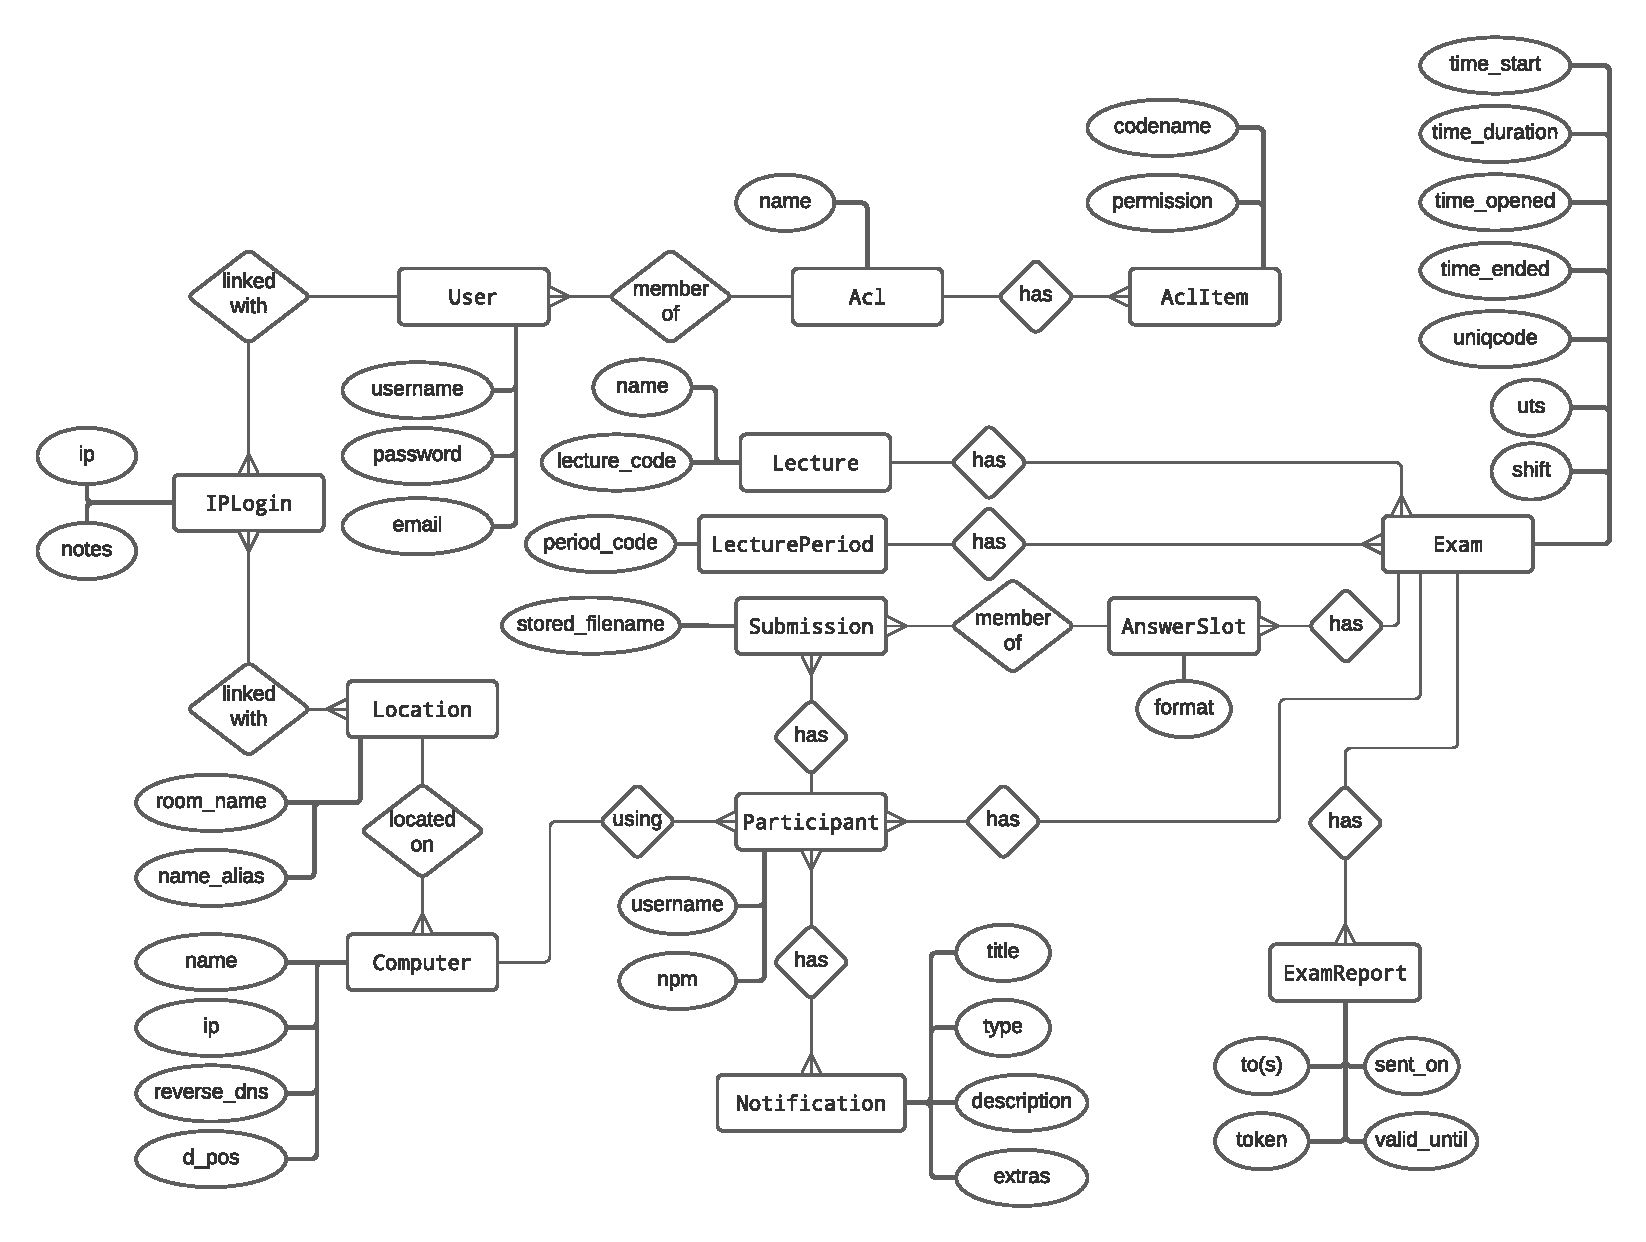
\includegraphics[width=1\paperwidth]{Gambar/erd-rev-b.pdf}
        \caption{Diagram \textit{ERD} untuk sistem aplikasi yang baru.}
        \label{fig:erd_overview}
    \end{sidewaysfigure}
    
    Perancangan basis data dimulai dengan merumuskan entitas yang dibutuhkan dan relasinya
    dengan entitas lainnya. Rumusan tersebut direpresentasikan dalam bentuk diagram relasi
    entitas atau ERD. Diagram ERD untuk aplikasi ini dapat dilihat pada Gambar \ref{fig:erd_overview}.
    Berdasarkan kebutuhan yang dianalisis pada bab sebelumnya, sistem membutuhkan empat belas
    entitas yang bertanggung jawab untuk merepresentasikan struktur data yang digunakan.
    Setiap entitas yang dibuat akan dibuat ulang representasinya dalam bentuk kelas pada
    sistem PHP dengan harapan membantu penanganan dan perancangan sistem REST API.
    
    Pembahasan akan dilanjutkan dengan menjelaskan satu per satu entitas yang ditunjukan
    pada diagram ERD. Pembahasan akan dimulai dengan entitas yang penulis kategorikan sebagai
    esensial untuk sistem terlebih dahulu, lalu dilanjutkan dengan entitas yang muncul dari
    analisis dari bab sebelumnya.
    
\subsubsection{User}
    % TODO: Figure mini user?.
    Entitas \texttt{User} merepresentasikan pengguna aplikasi. Entitas ini akan menyimpan informasi
    khusus seperti nama pengguna (\texttt{username}), kata sandi (\texttt{password}) dan email.
    Kolom \texttt{password} pada entitas ini akan di\textit{hash} menggunakan algoritma Blowfish
    dengan bantuan \textit{library} dari PHP dengan alasan keamanan.
    
    Entitas ini dinilai esensial karena entitas ini digunakan untuk melakukan otentikasi
    menuju panel admin. Entitas ini akan memiliki perlakuan khusus pada saat data
    dari entitas ini ditransmisikan ke sistem frontend. Otentikasi ini penting untuk
    mengkhususkan peran dari setiap pengguna.

\subsubsection{ACL dan ACLItem}
    \begin{figure}[H]
        \centering
        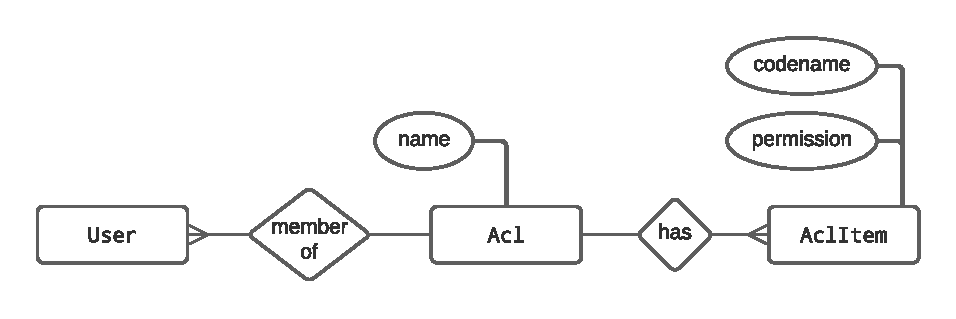
\includegraphics[width=0.75\paperwidth]{Gambar/erd-details/ERD--New - ACL & ACLItem.pdf}
        \caption{Potongan diagram entitas untuk \texttt{ACL} dan \texttt{ACLItem}.}
        \label{fig:erd_acl-aclitem}
    \end{figure}
    
    Entitas \texttt{ACL} dan \texttt{ACLItem} adalah entitas yang menampung informasi 
    tentang peran dan izin untuk
    setiap pengguna, diperjelas pada Gambar \ref{fig:erd_acl-aclitem}. 
    \texttt{ACL} menyimpan grup utama dari \texttt{ACLItem}, atau dapat kita 
    sebut sebagai peran.
    Sedangkan \texttt{ACLItem} menyimpan informasi izin untuk setiap nama 
    kasus (\texttt{codename}) yang diperbolehkan.
    
    \begin{table}[H]
        \centering
        \begin{tabular}{|l|l|l|}
        \hline
        Label & Deskripsi & Nilai Biner \\ \hline
        C     & Buat      & \texttt{0001}        \\ \hline
        R     & Baca      & \texttt{0010}        \\ \hline
        U     & Perbarui  & \texttt{0100}        \\ \hline
        D     & Hapus     & \texttt{1000}        \\ \hline
        \end{tabular}
        \caption{Tabel representasi nilai biner pada kolom \texttt{permission} di entitas \texttt{ACLItem}}
        \label{tab:aclitem_level}
    \end{table}
        
    
    Perizinan direpresentasikan dengan menggunakan sistem biner yang disimpan pada database sebagai angka.
    Representasi biner ini terdiri dari label CRUD, dengan C adalah Buat (\textit{Create}), R adalah
    Baca (\textit{Read}), U adalah Perbaharui (\textit{Update}) dan D adalah Hapus (\textit{Delete}).
    Label tersebut kemudian diberikan tempat khusus pada bitstring sebelum akhirnya dikonversi
    sebagai angka. Nilai-nilai tersebut dapat dilihat pada tabel \ref{tab:aclitem_level}.
    
    % TODO: ganti jadi rumus math yang bener.
    Sebagai contoh, seorang pengguna dapat \textbf{membuat}, \textbf{membaca}, \textbf{memperbarui}
    namun tidak dapat menghapus sebuah entri. Nilai dari tabel \ref{tab:aclitem_level} digabungkan
    dengan operator \texttt{OR} untuk setiap izin yang diberikan.
    Dengan begitu, nilai \texttt{permission} yang diberikan adalah
    $0001 \vee 0010 \vee 0100 \vee 0000 = 0111$ dengan \texttt{0111} disimpan sebagai 7 pada database.
    
    Pengecekan izin \texttt{permission} dilakukan dengan memanfaatkan operator \texttt{AND} antara 
    nilai pada kolom \texttt{permission} dengan nilai \texttt{permission} yang diekspektasikan, lalu
    dibandingkan dengan nilai ekspektasi.
    Sebagai contoh, sistem perlu mengecek apakah pengguna dapat membuat sebuah entri. 
    Sistem dapat melakukan pengecekkan dengan melakukan operasi \texttt{AND} pada nilai 
    \texttt{permission} yang ada saat ini (\texttt{0111}) dengan nilai \texttt{permission} yang
    diekspektasi (\texttt{0010}): $0111 \wedge 0010 = 0010$ dengan hasil sama seperti ekspentasi.
    Dengan begitu sistem dapat menilai bahwa pengguna tersebut memiliki izin untuk melakukan hal
    tersebut.
    
\subsubsection{IPLogin}
    \begin{figure}[H]
        \centering
        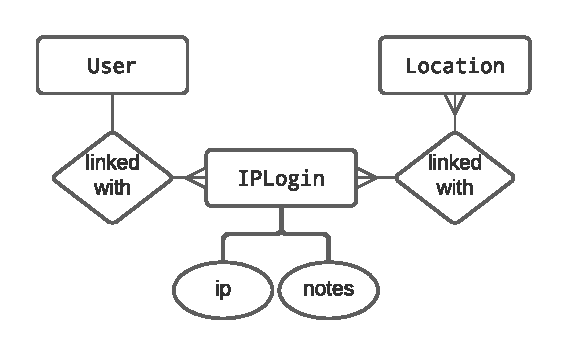
\includegraphics{Gambar/erd-details/ERD--New - IPLogin.pdf}
        \caption{Potongan diagram entitas untuk \texttt{IPLogin}.}
        \label{fig:erd_iplogin}
    \end{figure}
    Entitas \texttt{IPLogin} digunakan untuk melakukan otentikasi semi-otomatis dengan memanfaatkan IP
    pengguna pada lab, ditautkan dengan sebuah akun pengguna dengan peran yang terbatas (hanya
    dapat melihat dan mengubah entitas tertentu), diperjelas pada Gambar \ref{fig:erd_iplogin}.
    Entitas menyimpan informasi IP, tautan pada pengguna dan lokasi-lokasi, serta catatan khusus
    tentang penautan tersebut. 
    
    Entitas ini memiliki hubungan \textit{many-to-many} dengan entitas \texttt{Location}. Relasi
    ini diharapkan agar Tim Admin dapat melakukan pengaturan komputer master untuk melihat 
    seluruh ujian yang aktif pada ruangan tertentu tanpa harus membuatkan akun khusus 
    tertentu pada sistem. Tim Admin dapat dengan mudah menautkan sejumlah ruangan yang diinginkan
    dengan akun yang memiliki peranan terbatas yang sudah ada sebelumnya.
    
    Entitas ini dinilai cukup esensial karena berhubungan dengan sistem otentikasi yang membatasi
    pengguna untuk melakukan aksi tertentu di admin panel.
    
\subsubsection{Location dan Computer}
    \begin{figure}
        \centering
        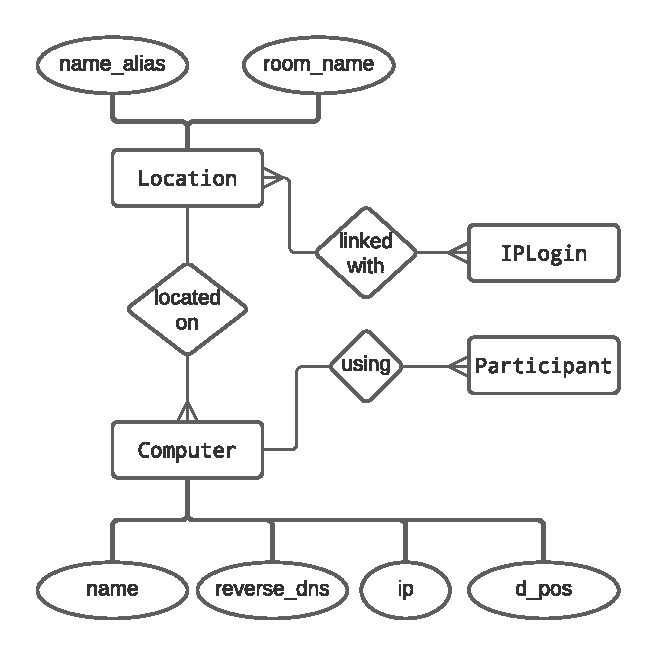
\includegraphics{Gambar/erd-details/ERD--New - Location & Computer.pdf}
        \caption{Potongan diagram entitas untuk \texttt{Location} dan \texttt{Computer}.}
        \label{fig:erd_location-computer}
    \end{figure}
    
    Entitas \texttt{Location} dan \texttt{Computer} menyimpan informasi tentang lokasi (ruagan) dan
    daftar pada komputer tersebut sebelum nantinya dihubungkan dengan entitas lainnya. Hubungan
    antara kedua entitas tersebut dapat diperhatikan pada potongan diagram entitas di gambar
    \ref{fig:erd_location-computer}.
    
    Entitas \texttt{Location} menyimpan informasi lokasi dan ruangan tempat peserta dapat mengikuti
    ujian. Pada entitas ini, informasi yang disimpan adalah nama ruangan tersebut dan nama lain
    dari ruangan tersebut. Berdasarkan survei lapangan, setiap ruangan memiliki nama lain, sehingga
    kolom \texttt{name\_alias} ditambahkan. Sedangkan nama ruangan disimpan pada kolom \texttt{room\_name}.
    
    Entitas \texttt{Computer} mendefinisikan komputer yang terdapat pada lokasi tersebut. Oleh karena
    itu hubungan yang dimiliki dengan entitas \texttt{Location} adalah \textit{one-to-many}.
    Entitas ini menyimpan informasi berupa nama komputer (\textit{name}), IPnya (\textit{ip}),
    nama FQDN (\textit{Fully Qualified Domain Name}) atau domain dari komputer tersebut (\textit{reverse\_dns}),
    dan detil letak posisi dari komputer tersebut pada peta ruangan (\textit{d\_pos}).
    
    Kolom \textit{d\_pos} digunakan untuk menyimpan informasi letak komputer pada peta dalam bentuk
    JSON. Bentuk format ini digunakan karena data ini digunakan hanya pada sistem frontend. Dengan
    kesepakatan yang diharapkan cukup fleksibel, maka bentuk pemosisian ini akan disimpan dalam 
    bentuk JSON.
    
    Kolom \textit{ip} digunakan untuk menautkan sebuah komputer dengan IP, sehingga tabel otentikasi
    yang digunakan oleh peserta dapat langsung merujuk pada entitas ini. Setiap komputer peserta
    yang ingin digunakan akan didaftarkan pada entitas ini. Untuk saat ini, karena survei lapangan
    menunjukan bahwa versi IP yang digunakan adalah versi 4, maka fokus aplikasi saat ini akan
    menggunakan IPv4.
    
    Selain itu, terdapat kolom \textit{reverse\_dns} yang digunakan untuk menyimpan informasi nama domain dari
    komputer tersebut. Kolom ini diharapkan dapat membantu Tim Admin dan pengembang aplikasi
    berikutnya untuk melakukan \textit{debugging} dan kebutuhan API lainnya. Nama domain ini didapatkan dari
    LDAP yang digunakan oleh Server Windows untuk melakukan auditing objek mereka. Komputer yang
    terhubung dengan Active Directory milik Lab akan terdaftar pada sistem internal LDAP milik Windows
    Server yang nantinya akan diberikan domain khusus untuk komputer tersebut.

\subsubsection{Lecture dan LecturePeriod}

    \begin{figure}
        \centering
        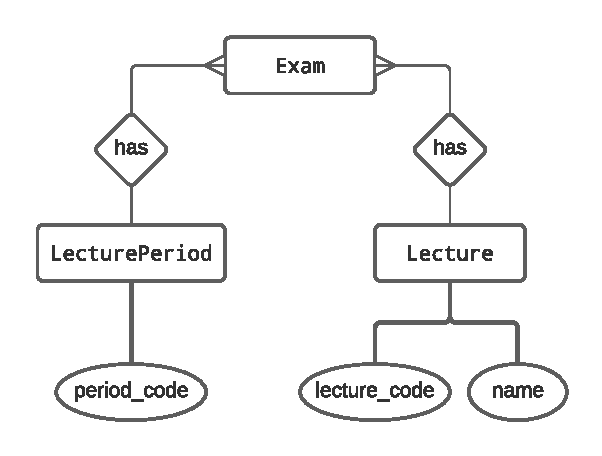
\includegraphics{Gambar/erd-details/ERD--New - Lecture & LecturePeriod.pdf}
        \caption{Potongan diagram entitas untuk \texttt{Lecture} dan \texttt{LecturePeriod}}
        \label{fig:erd_lecture-lectureperiod}
    \end{figure}

    Entitas \texttt{Lecture} dan \texttt{LecturePeriod} menyimpan informasi tentang mata kuliah
    dan periode tahun ajar mata kuliah bersangkutan pada ujian tertentu. Hubungan antara kedua
    entitas tersebut terhadap entitas \texttt{Exam} dapat dilihat pada potongan diagram entitas di 
    gambar \ref{fig:erd_lecture-lectureperiod}.  Entitas \texttt{Lecture} menyimpan informasi nama
    mata kuliah beserta kodenya, dan \texttt{LecturePeriod} menyimpan informasi tahun ajaran
    dalam bentuk kode.
    
    \begin{table}[]
        \centering
        \begin{tabular}{|l|l|}
        \hline
        Nilai & Tipe Semester \\ \hline
        1     & Ganjil        \\ \hline
        2     & Genap         \\ \hline
        3     & Pendek        \\ \hline
        \end{tabular}
        \caption{Definisi tipe semester dengan nilainya untuk kolom
            \texttt{period\_code} pada entitas \texttt{LecturePeriod}}
        \label{tab:lecture-periode}
    \end{table}
    
    Kode tersebut terdiri dari lima digit angka yang terdiri dari tahun ajar dan tipe semester
    yang sedang berjalan. Empat digit pertama adalah tahun ajar, dan satu digit terakhir adalah
    tipe semester. Tipe semester dan nilai representasinya dapat dilihat lebih jelas pada tabel
    \ref{tab:lecture-periode}.
    
    Sebagai contoh, semester ganjil pada tahun ajar 2016-2017 direpresentasikan sebagai
    \texttt{20161}. Empat digit pertama diambil dari tahun ajar pada tahun dimulai, 2016. Lalu
    berdasarkan tabel \ref{tab:lecture-periode}, semester ganjil memiliki nilai representasi
    1, sehingga kode untuk tahun ajar yang disimpan pada kolom \textit{period\_code} 
    adalah \texttt{20161}.
    

\subsubsection{Exam}
    \begin{figure}
        \centering
        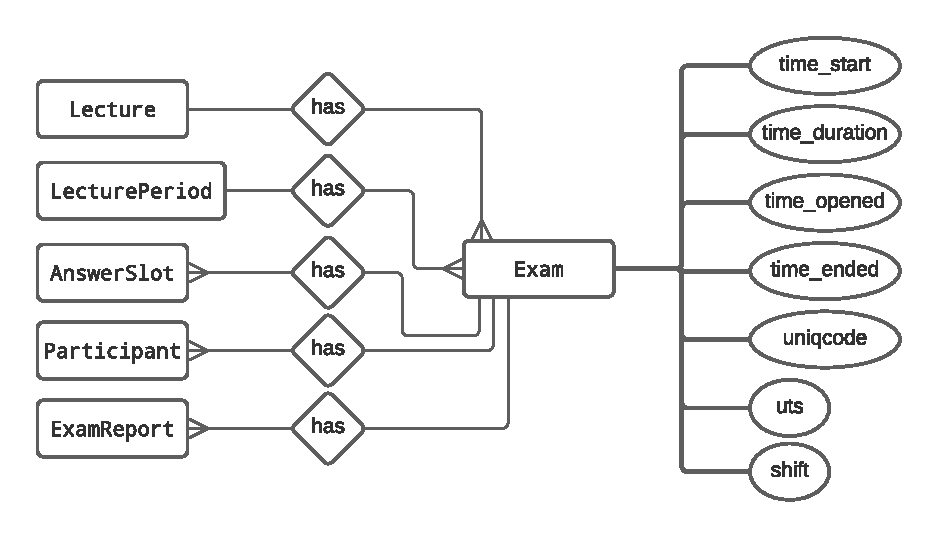
\includegraphics[width=0.75\paperwidth]{Gambar/erd-details/ERD--New - Exam.pdf}
        \caption{Potongan diagram entitas untuk \texttt{Exam}.}
        \label{fig:erd_exam}
    \end{figure}
    Entitas berikutnya yang akan dibahas adalah entitas \texttt{Exam}, dapat dilihat pada potongan
    gambar \ref{fig:erd_exam}. Entitas ini menyimpan informasi utama untuk ujian dan jadwalnya.
    Informasi jadwal disimpan pada kolom dengan \textit{prefix} \texttt{time\_}. Informasi dasar
    dari ujian tersebut disimpan dengan relasi langsung ke tabel lain seperti \texttt{Lecture},
    \texttt{LecturePeriod}, \texttt{AnswerSlot}, dan seterusnya. 
    
    Informasi yang cukup penting pada entitas ini terdapat pada kolom \texttt{uniqcode}. Kolom
    ini menyimpan informasi kode unik dari sebuah ujian yang kita gunakan untuk menyimpan informasi
    nama folder berkas ujian. Kode ini diharapkan terdiri dengan byte acak yang dibangkitkan dengan
    standar pengacakan untuk kriptografi. Pengacakan dengan standar tersebut diharapkan dapat
    memperkecil faktor kemungkinan serangan prediksi kode unik (\textit{guessing attack}).
    
    Pengecekan ujian yang aktif dilakukan dengan melakukan pengecekan pada kolom 
    \texttt{time\_start} dan \texttt{time\_ended}. Kolom \texttt{time\_start} menandakan
    informasi tentang kapan ujian \textbf{akan} dimulai. Kolom ini tidak menentukan kapan
    lembar jawaban dapat di\textit{submit} oleh peserta ujian. Sedangkan kolom \texttt{time\_ended}
    menandakan informasi tentang kapan lembar jawaban ditutup.
    
    Untuk membuka lembar jawaban, kolom \texttt{time\_opened} dan \texttt{time\_ended} harus diisi
    dengan informasi tanggal kapan lembar jawaban telah dibuka. Pada keadaan bawaan, normalnya
    kolom-kolom tersebut seharusnya memiliki nilai \texttt{NULL}. Pada saat Dosen Pengawas melakukan
    aksi membuka jawaban, maka kedua kolom tersebut harus diisi sesuai dengan durasi yang diberikan
    pada kolom \texttt{time\_duration}. Pengisian kolom \texttt{time\_opened} dam \texttt{time\_ended}
    diharapkan dapat mengurangi beban sistem untuk melakukan perhitungan secara terus menerus jika
    \texttt{time\_ended} tidak diberikan. Selain itu, dengan mengisi dua kolom tersebut secara
    simultan, diharapkan dapat mengurangi potensi masalah ujian lupa ditutup.
    
\subsubsection{}

\subsection{Rancangan REST API}
    % sistem otentikasi
    
    % desail url berdasarkan rest API
    
\subsection{Desain Kelas}
    % diagram kelas
    
\section{Perancangan Sistem Frontend}
    % diagram kelas dan file
    
    % Jelasin komponennya satu satu
\section{Perancangan Sistem CI/CD dan Unit Testing}
    % melakukan build pada saat commit
    % melakukan unit testing pada saat commit
    % unit testing yang dilakukan cuma buat 